\section{Model, problem and approach}
\label{sec:background}
%% In this section, we review the principles of general-purpose topic modeling with \lda~\cite{lda}, \tmlda~\cite{DBLP:conf/kdd/WangAB12} and \atam~\cite{atam2}.
%\subsection{Modeling topics with \lda and \atam}
\begin{table}[t!]
\centering
\caption{Mapping tweets to documents}
\label{tab:model:terms}
\begin{tabular}{|c|c|}
\hline
{\bf Term} & {\bf Description}\\
\hline
$\mf P$ & set of (tweet) posts\\
\hline
$\mf G$ & set of regions\\
\hline
$\mf T$ & set of time periods\\
\hline
$\mf P_g^t$ & posts from region $g$ during time $t$\\
\hline
$D_g^t$ & document-set built by mapping the content\\
& of each post $p\in \mf P_g^t$ to a document\\
\hline
$\Theta_g^t$ & ailment distribution vector for document-set\\
& $D_g^t$ of region $g$ during time $t$\\
\hline
$m$ & distance measure between distributions\\
\hline
\end{tabular}
\end{table}
Table~\ref{tab:model:terms} summarizes the terminology we use throughout this paper. By using suitable geographic granularity $g$ (country, state, county) and temporal granularity $t$ (week, fortnight and months), we build our document sets  $D_g^t$.
While LDA is successful at uncovering generic topics, its limitations at discovering
infrequent and specific topics such as health has already been shown \cite{atam2}.
The probabilistic \emph{Ailment Topic Aspect Model} (\atam) was designed 
specifically to uncover latent health-related topics present in a 
collection of tweets~\cite{atam2}. \atam achieves
remarkable improvement over LDA in discovering topics that correspond to 
ailments (in addition to discovering general topics). The topic distribution vector generated by \atam for a sample tweet is shown 
in Figure~\ref{fig:ldavsatam}. Note the stronger relevance to 
health--related matters in this vector than in the topic distribution vector 
generated by LDA for the same tweet.
While \atam is effective at modeling health-related topics, 
it is not designed to model topic transitions over time. 
\begin{figure}[t!]
\centering
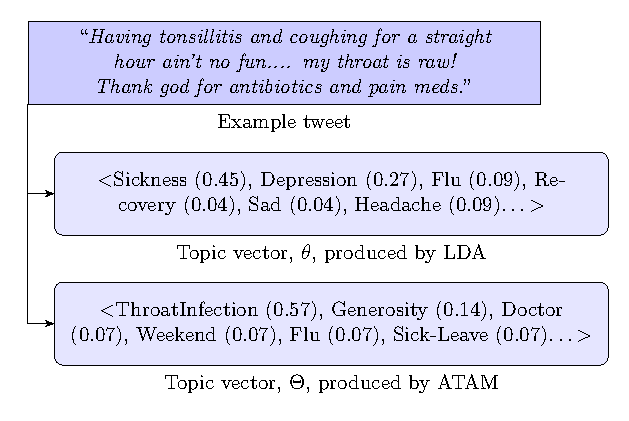
\includegraphics[width=0.45\textwidth]{tikz/exampleTweet3.pdf}
\caption{\lda vs \atam: Comparison of topic distributions for an example tweet.}
\label{fig:ldavsatam}
\end{figure}
\subsection{Ailment prediction problem}
\begin{figure}[b!]
\centering
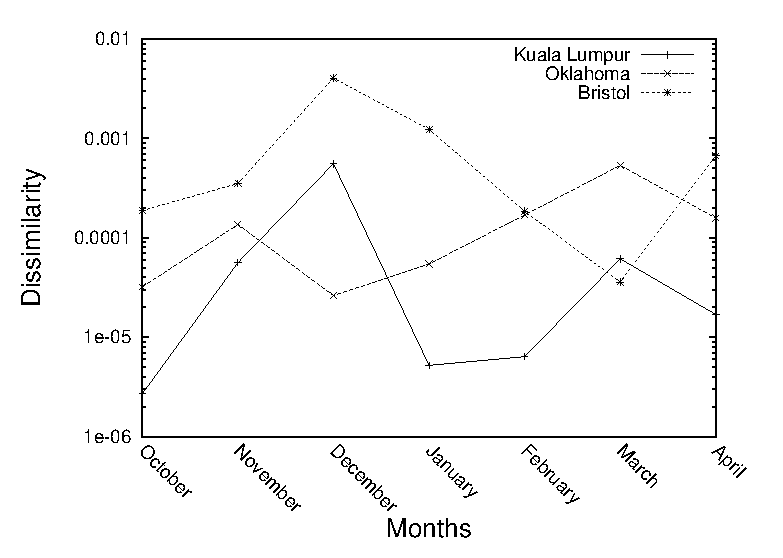
\includegraphics[width=0.45\textwidth]{gnuplot/distributiondifference/bhattacharyadistance.eps}
\caption{Topic transitions over time.}
\label{fig:ailmentsEvolve}
\end{figure}
In ~\cite{DBLP:conf/kdd/WangAB12}, \tmlda was introduced to extend \lda with modeling topic evolution over time. However, While being quite elegant in modeling general-purpose topics \tmlda is
not specialized to capture \texttt{\emph{health}} transitions over time.

Let $\Theta_g^t$ be a ailment distribution vector where the weight of each ailment is representative of the discourse density of ailment in the tweets originating from region $g$ during period $t$.
For a region $g$, the interval of time spanning a set of consecutive time periods $\{t_i,t_{i+1},\ldots\}$ during which discovered ailment distributions  $\{\Theta_g^{t_i},\Theta_g^{t_{i+1}},\ldots\}$
do not change appreciably forms a \season w.r.t. ailments. By definition, a \season is (nearly) homogeneous in terms
of ailments. In other words, the ailments evolve in a smooth fashion
within a \season and change abruptly across \season boundary. We posit that such \seasons exist after which they encounter \changes in ailment topic discussions. These \changes in ailment topic discussions 
may be caused by onset of the disease or some other external factors. Nevertheless, they are the interesting points for analyzing purposes.
As an example, in Figure~\ref{fig:ailmentsEvolve}, we show the difference between ailment distributions of consecutive months for 3 different regions Kuala Lumpur (a city in Indonesia), Oklahoma (a state in the USA), and Bristol (a city in the UK). The sharp peaks obtained validate the existence of time intervals that are homogeneous w.r.t. ailments.
\begin{algorithm}[t!]
\caption{TM-ATAM: \change Detection and Training Ailment Distribution Predictor}
\label{alg:tmatam}
\begin{algorithmic}[1]
 \ForAll {$g \in G$}\label{alg:line:start}
 \State Run ATAM on $D_g$\label{alg:line:atam}
 \ForAll  {$t \in \mf T$}:\label{alg:line:tstart}
 \ForAll {$z \in \mf Z$}:\label{alg:line:createThetaStart}
 \State $\Theta_g^t[z] \leftarrow 0$
 \EndFor
 \ForAll {$d \in D_g^t$}:
 \ForAll {$w \in d$}:
 \State $z \gets topic(w)$
 \State $\Theta_g^t[z] \gets \Theta_g^t[z] + \frac{1}{|d|\times |D_g^t|}$
 \EndFor
 \EndFor\label{alg:line:createThetaEnd}
 \EndFor
 \State $\displaystyle t_{c} = \argmax_t{\ m(\Theta_g^{t-1},\ \Theta_g^{t})}$\label{alg:line:ThetaDiff}
 \State $pre = [t_1\ ,\ t_{c-1}]$\label{alg:line:buildSeasonPre} 
 \State $post = [t_{c}\ , \ t_{|\mf T|}]$\label{alg:line:buildSeasonPost} 
 \ForAll {$s \in \{pre,\ post\}$}:\label{alg:line:predStart}
 \State $A_g^t\approx A_g^{t-1}.M$
 \State $M =(A_g^{t-1\intercal}A_g^{t-1})^{-1}A_g^{t-1\intercal}A_g^t$
 %\State $M = A_g^{t-1}\textsuperscript{\textdagger}A_g^t=(A_g^{t-1\intercal}A_g^{t-1})^{-1}A_g^{t-1\intercal}A_g^t$
 \EndFor\label{alg:line:predEnd}
\EndFor\label{alg:line:end}
\end{algorithmic}
\end{algorithm}

\label{subsec:problem}
{\bf Our problem:} Given a set of
documents $D_g^{t_{i-1}}$ formed by tweets originating from a region
$g \in G$ during time period $t_{i-1}$, predict $\Theta_g^{t_i}$, the
ailment distribution of documents in $D_g^{t_i}$, corresponding to
posts from $g$ in period $t_i$ from $\Theta_g^{t_{i-1}}$, the ailment
distribution of document $D_g^{t_{i-1}}$ corresponding to posts from
$g$ during period $t_{i-1}$.
\subsection{Modeling Health Topics over Time with \tmatam}
\label{subsec:model}
To solve our problem, we propose \tmatam that builds on top of \atam and \tmlda.
We first convert inferences of \atam over a single document to associate with a given set of documents $D_g^t$, an ailment
distribution, $\Theta_g^t$. We then go on to find \seasons. We model ailment transitions within each \season and when a \change is 
encountered we update these transitions.  This is a fresh departure
from existing solutions that operate in a \season-agnostic fashion\cite{DBLP:conf/kdd/WangAB12}.
\tmatam, at its heart, solves the following equation.
\begin{equation}
A_g^{t}\approx A_g^{t-1}.M^*
\end{equation}
where
\begin{equation}
A_g^{t-1}=\begin{pmatrix}\Theta_g^1\\\vdots\\\Theta_g^t\end{pmatrix},\,A_g^t=\begin{pmatrix}\Theta_g^2\\\vdots\\\Theta_g^{t+1}\end{pmatrix}
\end{equation}
$M^*$ is an unknown transition matrix which is obtained by solving the following least squares problem.
\[
M^*=\mathop{argmin}_M\|A_g^t- A_g^{t-1}.M\|_F
\]
Algorithm~\ref{alg:tmatam} contains the steps of our solution. It has 
two parts:  \change \emph{\texttt{detection}} and \emph{\texttt{ailment prediction}}. 
\paragraph{Change Point Detection}
We use $\mf Z$ to refer to the set of all health-related and
non-health related topics. For each region $g \in \mf G$
(Line~\ref{alg:line:start}) we first run \atam over the full time
period $D_g$ (Line~\ref{alg:line:atam}).  Next for each period $t\in
\mf T$ (Line~\ref{alg:line:tstart}), we use the output of \atam over
$D_g$ to generate a topic distribution $\Theta_g^t$
(Lines~\ref{alg:line:createThetaStart}--
\ref{alg:line:createThetaEnd}).  We then examine the
\emph{Bhattacharyya Distance} between consecutive distributions
$\Theta_g^{t-1}$ and $\Theta_g^t$ of the region $g$ to identify the
most significant \change, $t_c$, for region $g$ (Line~\ref{alg:line:ThetaDiff}). The
time periods preceding and succeding \change are termed as \seasons.
\paragraph{Ailment Prediction}
In the second module of \tmatam algorithm, we predict distribution of ailments in twitter discourse ahead of time for each \season.
Lines~\ref{alg:line:predStart}--\ref{alg:line:predEnd} 
of Algorithm~\ref{alg:tmatam} outline the steps undertaken to identify the detection of ailments for intra-homogeneous periods.
